\section{Neural Geometry Fields (NGFs)}\label{Sec:MainPart}

Sivaram and colleagues divide the Neural Geometry Fields pipeline into three distinct stages.

First, they input a base mesh \( \Sigma \) and partition it into quadrangular patches.
From this, they construct a trainable feature field \( \Psi : \Sigma \to \mathbb{R}^F \), associating each patch with a set of features that describe its surface properties, where each feature consists of \( F \) real components.
In the second stage, they feed these features, along with the 3D positions of the mesh, into a neural network that computes the displacement for each point on the mesh.
They then apply the displacements to the base mesh, producing a transformed conventional triangle mesh.
Finally, they optimize the feature field and patches using an inverse rendering algorithm.

In the following sections, we explore each stage in greater detail and provide an example to clarify the process further.






\subsection{Surface Partitioning into Patches}

Sivaram and colleagues introduce a method for surface representation by partitioning a base mesh, denoted as $\Sigma$, into quadrilateral patches $\sigma$ (see Figure~2).  
The process begins by simplifying the input mesh using QSlim, a robust and scalable algorithm that preserves important topological features such as holes and intersections.  
Following simplification, adjacent triangles are greedily merged into near-rectangular quadrilaterals, removing non-manifold triangles in the process.  
This allows the method to handle non-manifold input surfaces and still produce a consistent quadrilateral patch structure.  
This produces a compact and regular representation of the surface geometry, with fewer patches and improved structure.  
\usetikzlibrary{calc, shapes.geometric, arrows.meta, decorations.pathreplacing, positioning, shapes}
\begin{figure}[ht]
  \centering
  \begin{adjustbox}{center}
  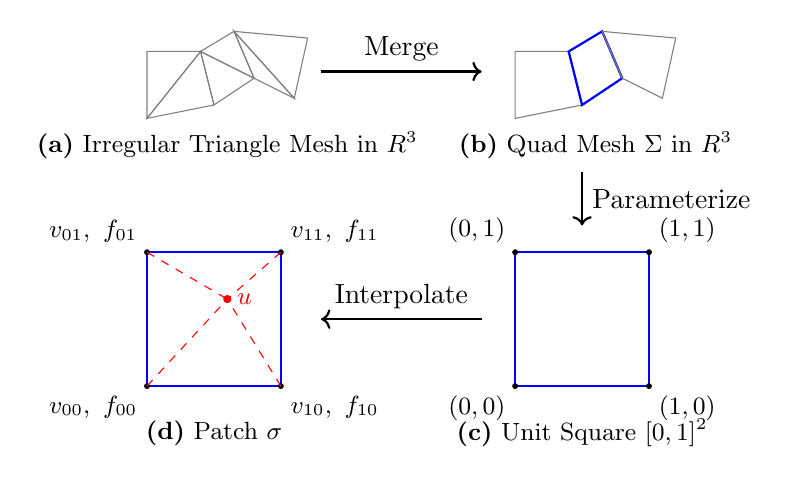
\begin{tikzpicture}[scale=0.85]

    % === Triangle Mesh (Left) ===
    \begin{scope}
      \coordinate (A) at (0,0);
      \coordinate (B) at (1,0.2);
      \coordinate (C) at (0.8,1);
      \coordinate (D) at (0,1);
      \coordinate (E) at (1.6,0.6);
      \coordinate (F) at (1.3,1.3);
      \coordinate (G) at (2.2,0.3);
      \coordinate (H) at (2.4,1.2);

      \draw[gray] (A) -- (B) -- (C) -- cycle;
      \draw[gray] (A) -- (C) -- (D) -- cycle;
      \draw[gray] (B) -- (E) -- (C) -- cycle;
      \draw[gray] (C) -- (E) -- (F) -- cycle;
      \draw[gray] (E) -- (G) -- (F) -- cycle;
      \draw[gray] (F) -- (G) -- (H) -- cycle;
      \node at (1.2, -0.4) {\small \textbf{(a)} Irregular Triangle Mesh in $\mathbb{R}^3$};
    \end{scope}

    % === Merge Arrow ===
    \draw[->, thick] (2.6,0.7) -- (5.0,0.7) node[midway, above] {Merge};

    % === Quadrilateral Mesh (Middle) ===
    \begin{scope}[xshift=5.5cm]
      \coordinate (A) at (0,0);
      \coordinate (B) at (1,0.2);
      \coordinate (C) at (0.8,1);
      \coordinate (D) at (0,1);
      \coordinate (E) at (1.6,0.6);
      \coordinate (F) at (1.3,1.3);
      \coordinate (G) at (2.2,0.3);
      \coordinate (H) at (2.4,1.2);

      \draw[gray] (A) -- (B) -- (C) -- (D) -- cycle;
      \draw[blue, thick] (B) -- (E) -- (F) -- (C) -- cycle; % highlighted patch
      \draw[gray] (E) -- (G) -- (H) -- (F) -- cycle;

      \node at (1.2, -0.4) {\small \textbf{(b)} Quad Mesh $\Sigma$ in $\mathbb{R}^3$};
    \end{scope}

    % === Down Arrow to Unit Square ===
    \draw[->, thick] (6.5,-0.8) -- (6.5,-1.6) node[midway, right] {Parameterize};

    % === Unit Square (Right) ===
    \begin{scope}[xshift=5.5cm, yshift=-4.0cm]
      \draw[blue, thick] (0,0) rectangle (2,2);
      \filldraw[black] (0,0) circle (1pt) node[anchor=north east] {\small $(0,0)$};
      \filldraw[black] (2,0) circle (1pt) node[anchor=north west] {\small $(1,0)$};
      \filldraw[black] (0,2) circle (1pt) node[anchor=south east] {\small $(0,1)$};
      \filldraw[black] (2,2) circle (1pt) node[anchor=south west] {\small $(1,1)$};
      \node at (1,-0.7) {\small \textbf{(c)} Unit Square $[0,1]^2$};
    \end{scope}

    % === Left Arrow to Feature Field ===
    \draw[->, thick] (5.0,-3) -- (2.6,-3) node[midway, above] {Interpolate};

    % === Feature Field (Left) ===
    \begin{scope}[yshift=-4.0cm]
      \draw[blue, thick] (0,0) rectangle (2,2);

      % Corner features (bold vectors), with f00 label moved outward
      \filldraw[black] (0,0) circle (1pt) node[anchor=north east] {\small $\bm{v_{00}},\ \bm{f_{00}}$};
      \filldraw[black] (2,0) circle (1pt) node[anchor=north west] {\small $\bm{v_{10}},\ \bm{f_{10}}$};
      \filldraw[black] (0,2) circle (1pt) node[anchor=south east] {\small $\bm{v_{01}},\ \bm{f_{01}}$};
      \filldraw[black] (2,2) circle (1pt) node[anchor=south west] {\small $\bm{v_{11}},\ \bm{f_{11}}$};

      % Interpolation point (u)
      \filldraw[red] (1.2,1.3) circle (1.5pt) node[right] {\small $\bm{u}$};

      % Lines from corners to interpolation point
      \foreach \x/\y in {0/0, 2/0, 0/2, 2/2} {
        \draw[dashed, red] (\x,\y) -- (1.2,1.3);
      }

      % Patch label
      \node at (1,-0.7) {\small \textbf{(d)} Patch $\sigma$};
    \end{scope}
    
  \end{tikzpicture}
  \end{adjustbox}
  \caption{Surface processing pipeline: The irregular triangle mesh is simplified and merged into a quadrilateral mesh $\Sigma$. A quadrilateral patch is extracted, which is then parameterized over the unit square $[0,1]^2$. This parameterization facilitates both geometric and feature field interpolation, with feature values interpolated at the patch's corners and at an arbitrary point $\bm{u}$. Inspired by~\cite{sivaram2024}.}
  \label{fig:surface_processing_pipeline}
\end{figure}
By relying on quadrilateral patches instead of a fully triangulated mesh, the method reduces the overall patch count $|Q|$ and simplifies the interpolation domain for later processing.  
This compression not only reduces storage requirements but also provides the foundation for an efficient and structured interpolation framework.  

To ensure smooth and consistent interpolation, each patch $\sigma$ must be diffeomorphic to the unit square $[0,1]^2$, meaning there exists a smooth, bijective mapping with a smooth inverse between the patch and the unit square.  
The four corner vertices of a patch are mapped as:
\[(0,0)\rightarrow v_{00}, \quad (1,0)\rightarrow v_{10}, \quad (0,1)\rightarrow v_{01}, \quad (1,1)\rightarrow v_{11}\]

To map an arbitrary point $u = (u_x, u_y)$ within the unit square to its corresponding location on the surface patch $\sigma$, bilinear interpolation is applied:  
\[\sigma(u) = (1 - u_y)((1 - u_x)v_{00} + u_x v_{10}) + u_y((1 - u_x)v_{01} + u_x v_{11}) \tag{1}\]  
This yields a continuous and smooth surface.  
Conceptually, this bilinear interpolation can be thought of as first interpolating along one axis (e.g., horizontal), then the other.  
The same interpolation strategy is used to propagate feature vectors defined at each patch corner.  

Each patch corner is associated with a high-dimensional learnable feature vector.  
In the configuration used by Sivaram et al., each vector has 20 dimensions, acting as a localized descriptor of geometric or semantic properties.  
The interpolated feature value $\Psi(u)$ for a point $u$ inside a patch is computed using bilinear blending:  
\[\Psi(u) = (1 - u_y)((1 - u_x)f_{00} + u_x f_{10}) + u_y((1 - u_x)f_{01} + u_x f_{11}) \tag{2}\]

The feature field $\Psi: \Sigma \rightarrow \mathbb{R}^F$ (with $F = 20$ in the authors' setup) allows the model to smoothly interpolate semantic information across the surface.  
These features, interpolated at arbitrary points on the patch, can be sampled across the surface for later neural processing stages.  

The complete set of mesh vertices and their associated features is defined as:  
\[V = \bigcup_\sigma \{v_{00}, v_{10}, v_{01}, v_{11}\}, \quad F = \bigcup_\sigma \{f_{00}, f_{10}, f_{01}, f_{11}\}\]  

These values are bilinearly interpolated across each patch and serve as input for the subsequent neural deformation stage.  
The surface layout defined in this step provides a structured yet flexible representation that supports efficient learning and reconstruction.  

The following section describes how this patch-based representation is used to generate detailed geometry through a neural deformation model, including the role of tessellation, feature encoding, and the architecture of the MLP.  





\subsection{Mesh Extraction from Neural Geometry Fields}

Building on the structured base mesh and a learned per-patch feature field, Sivaram et al.\ propose a neural surface deformation framework that reconstructs high-fidelity geometry by predicting local displacements.  
Each point $u \in [0,1]^2$ within a patch domain is mapped through a learned displacement field computed by a multi-layer perceptron ($\text{MLP}_\theta$), conditioned on both geometry and semantic features.  





\subsubsection{Patch-Based Sampling and Feature Encoding}

To extract a high-resolution mesh from the learned neural geometry field, Sivaram et al.\ subdivide the surface of the structured base mesh into parametric patches.  
Each quadrilateral face defines a patch $\sigma$ that maps the unit square domain $[0,1]^2$ onto a corresponding portion of the 3D surface using bilinear interpolation.  
Within each patch, a regular sampling grid of resolution $k \times k$ is established, creating a set of 2D coordinates $u_{ij} \in [0,1]^2$, where $i,j \in \{0, \ldots, k-1\}$.  

Within each patch, a regular $k \times k$ sampling grid is defined, producing 2D coordinates $u_{ij} \in [0,1]^2$, where $i,j \in \{0,\ldots,k-1\}$.  
For each sample $u_{ij}$, two interpolations are performed:  
\begin{enumerate}
    \item The base 3D position $\sigma(u_{ij})$,  
    \item The interpolated feature vector $\Psi(u_{ij})$.
\end{enumerate}

To capture fine-scale surface details, each MLP input includes a high-frequency positional encoding of the 3D position $v = \sigma(u)$ and the feature vector $f = \Psi(u)$.  
This encoding is defined as:  
\[\text{enc}(v, f) = (\sin(2^0 v), \cos(2^0 v), \ldots, \sin(2^L v), \cos(2^L v), f) \tag{3}\]  
where $L$ controls the number of frequency bands, and thereby the positional encoding resolution.  
This concatenated representation combines geometric and semantic information in a form well-suited for learning complex surface deformations~\cite{mildenhall2020nerf}.  
Sivaram et al.\ set $L = 8$ in their configuration.  
\begin{figure}[ht]
  \centering
  \begin{adjustbox}{center}
  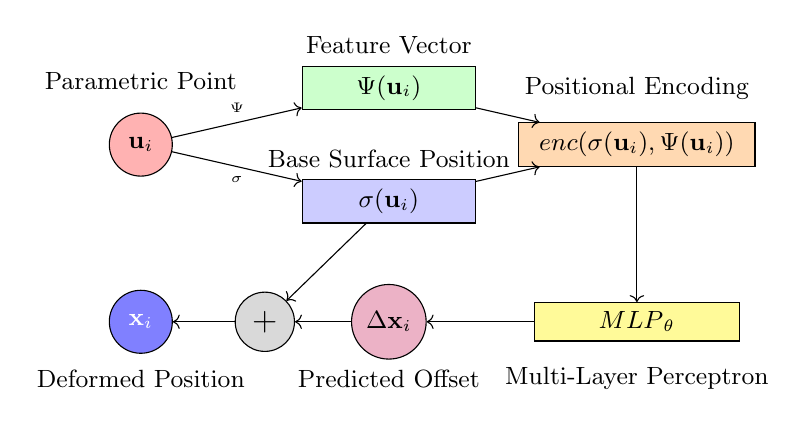
\begin{tikzpicture}[scale=0.9]

    % Sample point u_i
    \node[draw, circle, fill=red!30, minimum size=0.8cm] (u) at (0,0) {\small $\mathbf{u}_i$};
    \node at (0,0.9) {\small Parametric Point};

    % Psi(u)
    \node[draw, rectangle, fill=green!20, minimum width=2.2cm] (psi) at (3.5,0.8) {\small $\Psi(\mathbf{u}_i)$};
    \node at (3.5,1.4) {\small Feature Vector};

    % Sigma(u)
    \node[draw, rectangle, fill=blue!20, minimum width=2.2cm] (sigma) at (3.5,-0.8) {\small $\sigma(\mathbf{u}_i)$};
    \node at (3.5,-0.2) {\small Base Surface Position};

    % Encoding node
    \node[draw, rectangle, fill=orange!30, minimum width=3cm] (enc) at (7,0) {\small $\text{enc}(\sigma(\mathbf{u}_i), \Psi(\mathbf{u}_i))$};
    \node at (7,0.8) {\small Positional Encoding};

    % MLP node
    \node[draw, rectangle, fill=yellow!40, minimum width=2.6cm] (mlp) at (7,-2.5) {\small $\text{MLP}_\theta$};
    \node at (7,-3.3) {\small Multi-Layer Perceptron};

    % Displacement vector
    \node[draw, circle, fill=purple!30, minimum size=0.8cm] (dx) at (3.5,-2.5) {\small $\Delta \mathbf{x}_i$};
    \node at (3.5,-3.3) {\small Predicted Offset};

    % Plus node for summing sigma(ui) and delta_x (smaller + symbol)
    \node[draw, circle, fill=gray!30, minimum size=0.6cm] (plus) at (1.75,-2.5) {\large $+$};

    % Final position
    \node[draw, circle, fill=blue!50, text=white, minimum size=0.8cm] (x) at (0,-2.5) {\small $\mathbf{x}_i$};
    \node at (0,-3.3) {\small Deformed Position};

    % Arrows
    \draw[->] (u) -- (psi) node[midway, above] {\tiny $\Psi$};
    \draw[->] (u) -- (sigma) node[midway, below] {\tiny $\sigma$};
    \draw[->] (sigma) -- (enc);
    \draw[->] (psi) -- (enc);
    \draw[->] (enc) -- (mlp);
    \draw[->] (mlp) -- (dx);
    \draw[->] (sigma) -- (plus);
    \draw[->] (dx) -- (plus);
    \draw[->] (plus) -- (x);

  \end{tikzpicture}
  \end{adjustbox}
  \caption{Neural displacement pipeline for a sampled point $\mathbf{u}_i$. The point is mapped to a corresponding feature vector $\Psi(\mathbf{u}_i)$ and a base surface position $\sigma(\mathbf{u}_i)$. These inputs are passed through a positional encoding and a learned MLP to produce a displacement vector $\Delta \mathbf{x}_i$. The final deformed position $\mathbf{x}_i$ is obtained by adding the base position and the predicted offset, shown by the plus symbol.}
  \label{fig:neural_displacement}
\end{figure}





\subsubsection{Neural Surface Deformation with MLP}

The displacement of a point $u \in [0,1]^2$ on patch $\sigma$ is computed via the MLP applied to the encoded position and features.  
The final deformed position $\Lambda(u)$ is given by:  
\[\Lambda(\mathbf{u}) = \sigma(\mathbf{u}) + \text{MLP}_\theta \circ \text{enc}(\sigma(\mathbf{u}), \Psi(\mathbf{u})) \tag{4}\]
This formulation enables local, learned deformations of the base mesh, capturing geometric details beyond the coarse patch approximation.  





\subsubsection{Objective Function}

In contrast to conventional inverse rendering pipelines that rely solely on image-based supervision, our method benefits from direct access to attributes of the reference geometry. 
Among these, we utilize surface normal vectors as a reliable signal for guiding local shape reconstruction. 
Given the deformed surface produced by the neural deformation function $\Lambda(u)$, we evaluate differentiable vertex normals on the sampled mesh using standard geometric operations, specifically, cross products of adjacent triangle edges. 
During rasterization, these per-vertex normals are interpolated across fragments to produce normal vector frame buffers $N(\cdot)$ for both the reference surface $\Gamma$ and the predicted surface $\Sigma$. 
Using these buffers, we define an image-space normal consistency loss that measures the per-pixel alignment between predicted and reference normals: 
\begin{equation} L = \frac{1}{|N(\cdot)|} \|N(\Gamma) - N(\Sigma)\|_1 + \frac{1}{|V|} \|L_V\|_1 \end{equation} 
This loss term enforces local geometric agreement in appearance and orientation, encouraging the network to reproduce surface detail. 
To promote a smooth and uniform distribution of vertices across the surface, we include a Laplacian smoothness term, defined as: 
\begin{equation} L_{\text{normal}} = \frac{1}{|N(\cdot)|} \|L_V\|_1 \end{equation} 
Where $L$ is the uniform mesh Laplacian operator applied to the set of uniformly sampled vertices $V$. 
This term regularizes the deformation by penalizing irregular local configurations, helping to avoid artifacts such as vertex clustering or excessive warping. 
The total objective function combines both terms: 
\begin{equation} L = L_{\text{normal}} + L_{\text{laplacian}} \end{equation} 
This unified formulation balances geometric accuracy with structural regularity, serving as the primary supervisory signal during training.





\subsubsection{Jittered Sampling for Detail and Regularization}

To enhance surface detail and improve gradient flow during training, Sivaram et al.\ introduce a jittering strategy, which slightly randomizes the sampling positions within each patch.  
Normally, sampling would occur on a perfectly regular grid across the surface, meaning each sampled point lies at a predictable, evenly spaced coordinate (e.g., every $1/10$th of the patch width).  
However, such uniform sampling can lead to aliasing artifacts and limited expressiveness, especially when the surface has fine-grained or high-frequency geometric details.  

To address this, the authors perturb each interior sample point (i.e., points not lying on the patch boundary) by a small random offset.  
More specifically, each 2D point $u \in [0,1]^2$ is randomly shifted by a vector drawn from a uniform distribution over a small disk of radius $\omega$.  
This is written as $u \sim u + D(\omega)$, where $D(\omega)$ represents a uniform sampling over a disk centered at the origin.  
Visually, instead of forming a rigid grid, the sample points become slightly ``noisy,'' helping the model to better generalize and learn fine surface variations.  

Importantly, the jitter radius $\omega$ is kept small (less than half the grid spacing, $\omega < 0.5k^{-1}$) to avoid triangle fold-overs, a common issue in mesh generation where triangle edges cross over each other, causing rendering artifacts and invalid geometry.  
Additionally, to preserve seamless boundaries between neighboring patches, boundary samples are left untouched (i.e., $\omega=0$ at the edges), ensuring that patch edges still align precisely.  

This jittering acts as a form of regularization, helping the model to avoid overfitting to a rigid sampling pattern and instead learn a smoother and more flexible deformation field.  
It also encourages robustness in surface prediction, particularly in low-resolution cases, where sparse sampling would otherwise miss subtle details.  
\begin{figure}[ht]
  \centering
  \begin{adjustbox}{center}
  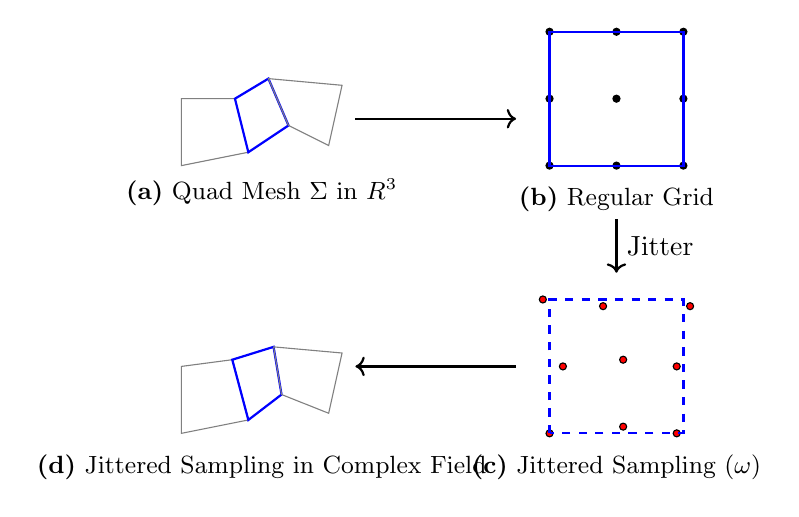
\begin{tikzpicture}[scale=0.85]

    % === (a) Irregular Triangle Mesh ===
    \begin{scope}
      \coordinate (A) at (0,0);
      \coordinate (B) at (1,0.2);
      \coordinate (C) at (0.8,1);
      \coordinate (D) at (0,1);
      \coordinate (E) at (1.6,0.6);
      \coordinate (F) at (1.3,1.3);
      \coordinate (G) at (2.2,0.3);
      \coordinate (H) at (2.4,1.2);

      \draw[gray] (A) -- (B) -- (C) -- (D) -- cycle;
      \draw[blue, thick] (B) -- (E) -- (F) -- (C) -- cycle; % highlighted patch
      \draw[gray] (E) -- (G) -- (H) -- (F) -- cycle;

      \node at (1.2, -0.4) {\small \textbf{(a)} Quad Mesh $\Sigma$ in $\mathbb{R}^3$};
    \end{scope}

    % Arrow
    \draw[->, thick] (2.6,0.7) -- (5.0,0.7) node[midway, above] {};

    % === (b) Regular Grid ===
    \begin{scope}[xshift=5.5cm]
      \foreach \x in {0,1,2} {
        \foreach \y in {0,1,2} {
          \filldraw[black] (\x, \y) circle (1.5pt);
        }
      }

      \draw[blue, thick] (0,0) rectangle (2,2);
      \node at (1,-0.5) {\small \textbf{(b)} Regular Grid};
    \end{scope}

    % Arrow
    \draw[->, thick] (6.5,-0.8) -- (6.5,-1.6) node[midway, right] {Jitter};

    % === (c) Jittered Grid ===
    \begin{scope}[xshift=5.5cm, yshift=-4.0cm]
      \foreach \x/\y in {
        0.0/0.0, 1.1/0.1, 1.9/0.0, 0.2/1.0,
        2.1/1.9, 1.1/1.1, 1.9/1.0, -0.1/2.0,
        0.8/1.9
      } {
        \filldraw[red, draw=black] (\x, \y) circle (1.5pt);
      }

      \draw[blue, thick, dashed] (0,0) rectangle (2,2);
      \node at (1,-0.5) {\small \textbf{(c)} Jittered Sampling ($\omega$)};
    \end{scope}

    % Arrow
    \draw[->, thick] (5.0,-3) -- (2.6,-3) node[midway, above] {};

    % === (d) Irregular Field + Jittered Points ===
    \begin{scope}[yshift=-4.0cm]
      
  \coordinate (A) at (0,0);
  \coordinate (B) at (1.000,0.200); %(1,0.2.0)
  \coordinate (C) at (0.760,1.100); %(0.8,1.0)
  \coordinate (D) at (0,1);
  \coordinate (E) at (1.496,0.580); %(1.6,0.6)
  \coordinate (F) at (1.377,1.292); %(1.3,1.3)
  \coordinate (G) at (2.2,0.3);
  \coordinate (H) at (2.4,1.2);

  \draw[gray] (A) -- (B) -- (C) -- (D) -- cycle;
  \draw[blue, thick] (B) -- (E) -- (F) -- (C) -- cycle; % highlighted patch
  \draw[gray] (E) -- (G) -- (H) -- (F) -- cycle;


  % === Jittered Points Mapped from (c) ===
  %\filldraw[red, draw=black] (1.000,0.200) circle (1.5pt); % (0.0, 0.0)
  %\filldraw[red, draw=black] (1.307,0.385) circle (1.5pt); % (1.1, 0.1)
  %\filldraw[red, draw=black] (1.496,0.580) circle (1.5pt); % (1.9, 0.0)
  %\filldraw[red, draw=black] (0.905,0.700) circle (1.5pt); % (0.2, 1.0)
  %\filldraw[red, draw=black] (1.377,1.292) circle (1.5pt); % (2.1, 1.9)
  %\filldraw[red, draw=black] (1.222,0.885) circle (1.5pt); % (1.1, 1.1)
  %\filldraw[red, draw=black] (1.450,0.880) circle (1.5pt); % (1.9, 1.0)
  %\filldraw[red, draw=black] (0.760,1.100) circle (1.5pt); % (-0.1, 2.0)
  %\filldraw[red, draw=black] (1.091,1.080) circle (1.5pt); % (0.8, 1.9)

  \node at (1.2, -0.5) {\small \textbf{(d)} Jittered Sampling in Complex Field};
\end{scope}


  \end{tikzpicture}
  \end{adjustbox}
  \caption{Progression from an irregular triangle mesh (a) to a regular sampling grid (b), jittered sampling within grid cells (c), and finally applying jittered sampling within a more complex field (d).}
  \label{fig:progression_sampling}
\end{figure}






\subsubsection{Mesh Construction and Differentiable Training}

Once the displaced 3D positions for all sample points have been computed using the MLP, the mesh is constructed by triangulating the sampled grid.  
Specifically, the $k \times k$ sampling grid within each patch defines $(k-1)^2$ square cells (quads), each of which is split into two triangles in a consistent pattern, similar to how elevation maps are converted into triangle meshes (often called height fields).  
Since each patch follows the same sampling and triangulation logic, and boundary points are shared consistently, the resulting mesh is semi-regular and coherent across patches, forming a watertight and well-structured surface.  

The MLP used by Sivaram and colleagues consists of two hidden layers with 64 neurons each and uses activation functions not explicitly specified by the authors.  
These functions introduce the non-linearities necessary for modeling complex deformation patterns, but their exact form is not detailed in the original description.  
Both the network parameters $\theta$ and the per-vertex feature vectors are optimized jointly during training.  

The training pipeline incorporates differentiable rendering using \texttt{NVDIFFRAST}, a GPU-accelerated rasterizer specifically designed for gradient-based optimization of 3D geometry and appearance~\cite{niemeyer2020}.  
Unlike traditional rendering methods, which are inherently non-differentiable and unsuitable for gradient-based learning, differentiable rendering allows loss gradients from image space to flow back into the 3D mesh and feature representations.  
This capability enables the system to iteratively update both geometry and per-patch features, improving alignment between the rendered outputs and the multi-view image supervision~\cite{kato2020}.  

To supervise this optimization process, the model relies on multi-view images, which are 2D projections of the object captured from various angles.  
These views serve as a comprehensive set of visual observations that constrain the reconstruction.  
Specifically, the 3D surface is rendered from 200 virtual camera viewpoints that simulate the perspectives from which the object could be observed.  
The camera viewpoints are uniformly distributed around the object to ensure comprehensive angular coverage, allowing the model to observe and reconstruct surface details from every side.  
This is essential for achieving a reconstruction that is geometrically accurate and consistent from every direction.  

For efficiency and improved training dynamics, these views are grouped into batches of 10, with each view incorporating three depth layers per pixel.  
This multi-layer rendering helps capture partial occlusions and complex visibility effects, such as surfaces seen through transparent or semi-transparent regions.  
By doing so, the model can reason more accurately about the 3D structure and avoid artifacts caused by occluded or ambiguous regions~\cite{burggraaff2018}.  

This comprehensive setup, combining differentiable rendering, multi-view supervision, and visibility-aware optimization, allows the learning algorithm to reconstruct detailed and consistent surface geometry.  
Optimization is performed using the Adam optimizer with a fixed learning rate of $10^{-3}$, providing a stable update mechanism for both the mesh deformation network and the associated feature vectors.  
The Adam optimizer is an adaptive method that adjusts the learning rate for each parameter based on the first and second moments of the gradients.  
This allows the optimizer to adaptively correct the learning rates during training, accelerating convergence while avoiding large, unstable updates.  
The fixed learning rate ensures stability during training, while the adaptive nature of Adam helps the model learn more efficiently from the gradients provided by the differentiable rendering process~\cite{kingma2017}.  





\subsubsection{Inverse Rendering}

To refine our neural surface representation beyond coarse geometry alignment, we employ an inverse rendering strategy based on rasterization.  
This approach allows us to optimize the appearance of the predicted surface to match the visual characteristics of the target data directly.  

Rather than relying on geometric proximity measures such as Chamfer distance or signed distance field (SDF) queries, which are often sensitive to sampling density and noise—our method leverages appearance-based supervision.  
This has proven more stable and effective, especially in complex regions with fine-scale details or partial visibility.  

At the heart of our optimization process lies a differentiable rasterizer that compares rendered images of the current mesh to the target observations from multiple viewpoints.  
This enables the computation of meaningful gradients that can be propagated back through the rendering pipeline.  

To further stabilize the training and encourage convergence, we adopt a coarse-to-fine optimization schedule.  
Starting with a lower tessellation resolution $k$, we progressively increase the sampling density, allowing the network to first capture global shape and then refine local details.  

At a fixed tessellation level $k$, the resulting mesh $M$ has a constant connectivity, defined by a regular triangulation of the sampled patch grid.  
Crucially, the vertex positions of this mesh are differentiable with respect to:
\begin{itemize}
    \item the patch corner positions $V$,
    \item the feature vectors $F$,
    \item and the neural deformation parameters $\theta$ of $\text{MLP}_\theta$.
\end{itemize}

This differentiability ensures that the inverse rendering pipeline produces useful and stable gradients, enabling the joint optimization of geometry and appearance.  
In this way, our method not only recovers high-quality surfaces but also aligns their rendered appearance with the target imagery, leading to visually and geometrically accurate reconstructions.  
